\documentclass[tikz,border=10pt]{standalone}
%%%<
\usepackage{verbatim}
%%%>
% \usetikzlibrary{shapes.geometric,backgrounds,
  % positioning-plus,node-families,calc}
% \tikzset{
%   basic box/.style = {
%     shape = rectangle,
%     align = center,
%     draw  = #1,
%     fill  = #1!25,
%     rounded corners},
%   header node/.style = {
%     Minimum Width = header nodes,
%     font          = \strut\Large\ttfamily,
%     text depth    = +0pt,
%     fill          = white,
%     draw},
%   header/.style = {%
%     inner ysep = +1.5em,
%     append after command = {
%       \pgfextra{\let\TikZlastnode\tikzlastnode}
%       node [header node] (header-\TikZlastnode) at (\TikZlastnode.north) {#1}
%       node [span = (\TikZlastnode)(header-\TikZlastnode)]
%         at (fit bounding box) (h-\TikZlastnode) {}
%     }
%   },
%   hv/.style = {to path = {-|(\tikztotarget)\tikztonodes}},
%   vh/.style = {to path = {|-(\tikztotarget)\tikztonodes}},
%   fat blue line/.style = {ultra thick, blue}
% }
\begin{document}
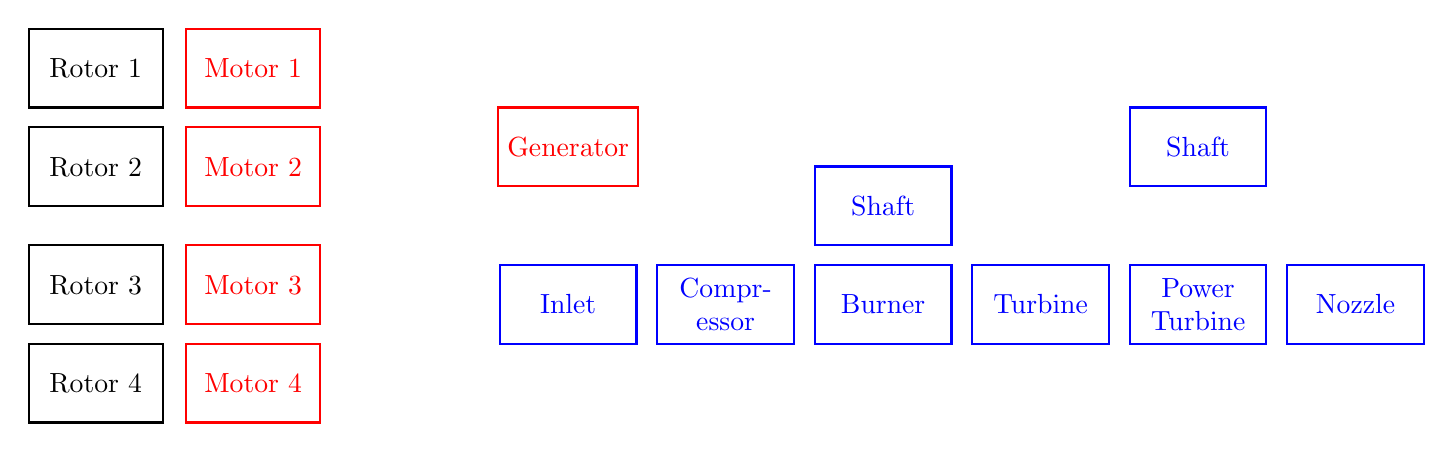
\begin{tikzpicture}[node distance = 1.2cm, thick, nodes = {align = center}, >=latex]

  \tikzstyle{rotor}=[draw, rectangle, minimum height=1cm, minimum width=1.7cm]
  \tikzstyle{elec}=[draw, rectangle, red, minimum height=1cm, minimum width=1.7cm]
  \tikzstyle{cycle}=[draw, rectangle, blue, minimum height=1cm, minimum width=1.7cm, text width=1.5cm]

  
  % \node[rotor] (r1) at (0,0) {Rotor 1};
  % \node[rotor] (r2) at (2,0) {Rotor 2};
  % \node[rotor] (r3) at (4,0) {Rotor 3};
  % \node[rotor] (r4) at (6,0) {Rotor 4};

  % \node[elec] (m1) at (0,-1.5) {Motor 1};
  % \node[elec] (m2) at (2,-1.5) {Motor 2};
  % \node[elec] (m3) at (4,-1.5) {Motor 3};
  % \node[elec] (m4) at (6,-1.5) {Motor 4};

  % \node[elec] (gen) at (3,-4.5) {Generator};

  % \node[cycle] (comp) at (3,-5.5) {Compressor};
  % \node[cycle] (burn) at (3,-6.5) {Burner};
  % \node[cycle] (turb) at (3,-7.5) {Turbine};
  % \node[cycle] (pt) at (3,-8.5) {Power Turbine};
  % \node[cycle] (nozz) at (3,-9.5) {Nozzle};
  % \node[cycle] (shaft) at (5,-6.5) {Shaft};



  \node[rotor] (r1) at (0,2.0) {Rotor 1};
  \node[rotor] (r2) at (0,0.75) {Rotor 2};
  \node[rotor] (r3) at (0,-0.75) {Rotor 3};
  \node[rotor] (r4) at (0,-2.0) {Rotor 4};

  \node[elec] (m1) at (2,2.0) {Motor 1};
  \node[elec] (m2) at (2,0.75) {Motor 2};
  \node[elec] (m3) at (2,-0.75) {Motor 3};
  \node[elec] (m4) at (2,-2.0) {Motor 4};

  \node[elec] (gen) at (6,1.0) {Generator};

  \node[cycle] (inlet) at (6,-1.0) {Inlet};
  \node[cycle] (comp) at (8,-1.0) {Compr-essor};
  \node[cycle] (burn) at (10,-1.0) {Burner};
  \node[cycle] (turb) at (12,-1.0) {Turbine};
  \node[cycle] (pt) at (14,-1.0) {Power Turbine};
  \node[cycle] (nozz) at (16,-1.0) {Nozzle};
  \node[cycle] (shaft) at (10,0.25) {Shaft};
  \node[cycle] (shaft) at (14,1.0) {Shaft};


  % \node[Minimum Width = loop, fill = yellow, below = of imp-sol] (rec-box)
  %   {rectangular box, and very wiiiiiiiiiiiiiiide\\2nd line};
  % \node[shift = (left:.5*x_node_dist)] at
  %   ($(imp-sol.west|-imp-sol.south)!.5!(rec-box.north west)$) (for-1)
  %   {formula 1};
  % \node[shift = (right:.5*x_node_dist)] at
  %   ($(imp-sol.east|-imp-sol.south)!.5!(rec-box.north east)$) (for-2)
  %   {formula 2};
  % \begin{scope}[on background layer]
  %   \node[fit = (for-1)(for-2)(imp-sol)(rec-box), basic box = blue,
  %     header = DMFT loop] (dmft-l) {};
  % \end{scope}
  % \path[very thick, blue, hv] (rec-box) edge[->] (for-1) edge[<-] (for-2)
  %                             (imp-sol) edge[->] (for-2) edge[<-] (for-1);

  % \node[east above = of dmft-l, basic box = green, header = DMFT prelude]
  %   (dmft-p) {Math and text math and text math and text\\
  %             math and text math and text math and text};
  % \node[north left = of dmft-l, basic box = green, header = $\rho$ update,
  %    shift = (down:y_node_dist)] (rho)
  %   {Much more text much more text\\much more text much more text};
  % \node[basic box = blue, header = DFT part, anchor = north] at
  %   (dmft-p.north-|rho) (dft) {So much text so much text so much text\\
  %   I think I need \texttt{tikz-lipsum}\\or something like that.};
  % \node[basic box = green, anchor = north] at
  %   ($(dft.north east)!.5!(dmft-p.north west)$) (upd) {update\\$math$};
  % \path[fat blue line, <-, dashed, vh] (rho) edge
  %   ({$(rho.south)!.5!(dmft-l.south)$}-|dmft-l.south west);
  % \path[fat blue line, ->]
  %   ({$(upd.south)!.5!(dmft-p.south)$}-|dmft-p.south west)
  %   coordinate (@) edge[<-, solid] coordinate[pos=.15] (@s)
  %   coordinate[pos=.9] (@e) (@-|dft.east)
  %   {[every edge/.append style=dashed, vh] (@s) edge[<-] (upd) (@e) edge (upd)}
  %   (h-rho) edge[dashed] (dft)
  %   ($(dmft-p.south)!.5!(dmft-p.south east)$)
  %   coordinate (@) edge (@|-dmft-l.north);
\end{tikzpicture}
\end{document}